%  Long-term memory 不是 key-value bank，却说使用同样的 update strategy，不成立
\section{Introduction}
\label{sec:intro}
\begin{wrapfigure}[17]{r}{0.57\textwidth}
\vspace{-.5cm}
        \hspace{+0.04cm}
        \centering
		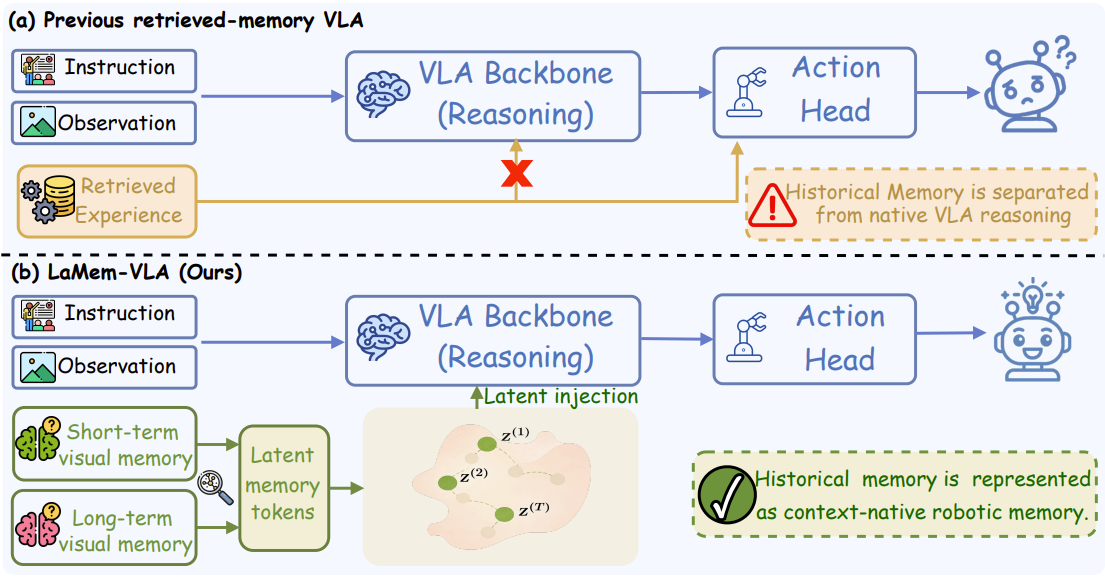
\includegraphics[width=0.99\linewidth]{figs/motivation.png}
\captionsetup{font=small,width=1\linewidth}
 \vspace{-.6cm}
	\caption{\small{Paradigm comparison of memory-augmented VLA Models. (a) Unlike previous VLA models that store historical experience in an auxiliary memory bank and consume retrieved memory as external policy-side context, (b) \ourmethod treats historical experience as context-native latent memory, which is stored, retrieved, and consumed in the model embedding space.
 }}
 \label{fig:motivation}
\end{wrapfigure}
Vision-language-action (VLA) models~\cite{black2024pi_0,kim2025openvla,liu2025rdt,zhen20243d} have become a promising paradigm for general robotic manipulation.
By combining the powerful capabilities of pretrained vision-language models~\cite{cheang2024gr,bai2023qwen,chen2024scaling} with policy learning~\cite{chi2025diffusion,zhang2025flowpolicy,octo_2023} on robotic data~\cite{o2024open,khazatsky2024droid,walke2023bridgedata,bu2025agibot}, they map visual observations and language instructions into executable action chunks.
Despite this progress, most existing VLA models~\cite{kim2025openvla,black2024pi_0,li2024cogact} implicitly rely on a Markovian assumption, predicting actions primarily from the current observation without considering temporal dependencies.
This simplification creates a \textit{temporal short-horizon bias}:
VLA models can react to the currently visible state, but fail to reason about previous state transitions, completed operation steps, and the current phase of a multi-step task.
As a result, these models especially struggle with long-horizon manipulation tasks.


% 但这会显著增加推理开销和内存占用。同时，这种做法还会使输入分布与 VLA 模型的预训练分布不一致
Recent efforts have sought to alleviate temporal short-horizon bias by augmenting VLA models~\cite{chi2025diffusion,li2024language,ze20243d} with historical context or memory mechanisms along two main axes.
\textit{\textbf{(i)}} One line of work incorporates short-horizon episode context by concatenating historical frames~\citep{li2024towards,fan2025interleave} or extending the input into a video sequence~\citep{li2025cronusvla,koo2025hamlet,hu2026resolving}.
Although such designs expose recent state changes, they incur computational and memory costs that grow with the context length, while the fixed temporal horizon imposes an inherent memory ceiling, causing potentially task-relevant evidence outside the window to be discarded.
\textit{\textbf{(ii)}} Another line of work~\citep{shi2025memoryvla,sridhar2025memer,li2026global} retrieves past trajectories or relevant historical tokens from an external memory bank to condition downstream action policies.
Although these methods demonstrate the value of historical experience for long-horizon manipulation, they still suffer from an architectural limitation: the historical memory is stored outside the model's native token space and consumed as auxiliary policy-side context after the VLA model reasoning.
This rigid separation prevents memory from being fluidly interleaved with the internal reasoning where the VLA model jointly perceives the scene, interprets the instruction, and resolves action queries before action formation.

This limitation raises a more fundamental question for memory-dependent VLA models: \textit{whether historical experience can be represented as context-native robotic memory, stored, retrieved, and consumed in the same continuous space where the VLA model already perceives, reasons, and acts?}
Latent embedding space~\cite{wang2026monet,yang2026machine,li2025latent,bai2026latent,zhang2025memgen,yu2026vismem,yu2026latent} offers a natural answer to this question. 
Modern VLA models already integrate visual observations and language instructions in a continuous token embedding space~\cite{zitkovich2023rt,kim2025openvla,black2024pi_0,li2024cogact}; therefore, robotic historical memory can be organized as machine-native latent memory tokens that are compatible with the internal reasoning process. 
Under this formulation, robotic memory becomes part of the model's operating context rather than an auxiliary scaffold attached after multimodal reasoning.
Long-horizon robotic manipulation also calls for two complementary forms of historical memory: \textbf{short-term memory} is visually dominant, preserving visually grounded evidence from the current episode, such as object locations and subtle state changes; \textbf{long-term memory} is semantically dominant, preserving task progress, contextual semantics, and action continuity across longer horizons.
Notably, their distinction lies in \textit{provenance and function} rather than in representation form: both are ultimately reconstructed as latent memory tokens that can be consumed by the VLA model in the latent space.
This leads to our pivotal research question:
\vspace{-0.4em}
\obsbox{
% \textcolor{black!70}{\faSearch[regular]}

\includegraphics[height=0.9em]{figs/question_icon2.png}~
\textit{How can we architect historical memory as a generative latent faculty, capable of fluidly reconstructing short-term visual evidence and long-term semantic evidence into compact memory tokens that interweave seamlessly with the VLA reasoning and action generation process?}}
\vspace{-0.2em}

To answer this question, we propose \ourmethod, a novel native latent memory framework for robotic manipulation, which explicitly organizes robotic history into two complementary memory vaults, and weaves dual-scale memory into the model reasoning for memory-augmented action generation.
At its core, \ourmethod closes the loop between latent memory weaving and action reasoning through four coordinated modules:
First, \ding{168} a \textbf{latent memory curator} factorizes past robotic experience into two complementary vaults: a short-term memory vault for recent visual evidence and a long-term memory vault for semantic and action-continuity evidence.
Second, during the action reasoning process, \ding{169} a \textbf{latent memory seeker} builds a context-aware query from the current multimodal cognition state (\ie, the visual and instruction tokens), and uses it to retrieve task-relevant historical evidence from dual memory vaults, grounding the present decision in past perceptual evidence and long-horizon semantic-action continuity. 
Third, \ding{170} a \textbf{latent memory condenser} compresses these potentially redundant retrieved evidence into fixed-length short-term and long-term latent memory tokens that are compatible with the VLA embedding space.
Finally, \ding{171} a \textbf{latent memory weaver} stitches these condensed memory tokens directly into the action reasoning sequence before action query tokens are resolved, allowing historical memory to participate in the same latent reasoning process as the current image, instruction, and action queries.
The resulting memory-grounded action queries condition a diffusion-based action expert~\cite{chi2025diffusion,peebles2023scalable} to generate temporally aware robotic action sequences.


% Through this curator--condenser--seeker--weaver pipeline, \ourmethod transforms historical memory from an external scaffold into an internal latent faculty. 
% The resulting memory tokens participate in self-attention with current image tokens, language tokens, and action query tokens, allowing past visual evidence and cognitive/action experience to shape action representations before they are decoded into continuous robot control.
We conduct comprehensive evaluations across two simulators (\ie, LIBERO~\cite{liu2023libero} and SimplerEnv-Bridge~\cite{li2025evaluating}).
On LIBERO, \ourmethod reaches an average success rate of \textbf{97.6}\%, outperforming MemoryVLA~\cite{shi2025memoryvla} by \textbf{1.1} points and our baseline CogACT~\cite{li2024cogact} by \textbf{4.4} points, while improving over \(\pi_0\)~\cite{black2024pi_0} by \textbf{3.5} points on the first four suites.
On SimplerEnv-Bridge, \ourmethod achieves \textbf{73.9}\% average success, surpassing our baseline CogACT~\cite{li2024cogact} by \textbf{16.6} points and \(\pi_0\)~\cite{black2024pi_0} by \textbf{4.7} points.
%In real-world evaluations, \ourmethod ranks best on both the general and long-horizon tasks, outperforming \(\pi_0\)~\cite{black2024pi_0} by xx\% and xx\%, respectively. 
These results indicate that weaving dual-scale latent robotic memory into VLA reasoning boosts the robustness of VLA models beyond policy-side memory conditioning, especially when action generation depends on task progress and historical cues.
One limitation of the current version is that the empirical validation is conducted in simulated environments. We are currently extending \ourmethod to real-world robot platforms, and the corresponding real-world experiments will be included in the next version.

In summary, our main contributions are as follows:
\begin{itemize}[leftmargin=*]
\item We introduce a new paradigm for robotic memory in VLA models: historical experience is treated as context-native latent memory, which is stored, retrieved, and consumed in the model embedding space, supporting scene perception, instruction understanding, and action-intent formation within the same latent reasoning process.
    \item We propose \ourmethod, a dual latent memory framework for robotic manipulation, which explicitly organizes robotic history into two complementary memory vaults, and weaves dual-scale memory into the model reasoning for memory-augmented action generation.
    \item We design a latent memory condensing mechanism, which transforms retrieved historical evidence into fixed-length latent short-term and long-term memory tokens that are compatible with the VLA model embedding space.
\end{itemize}
